% ============================================================
% CAPITOLO 5 - SCELTA DELL'ARCHITETTURA DEL MODELLO
% ============================================================

\section{Scelta dell'Architettura del Modello}

Una volta completata la pulizia e il bilanciamento del dataset, il passo successivo è la scelta del modello di classificazione. Il problema da risolvere è il seguente: data una sequenza di frame, ciascuno contenente le coordinate dei landmark estratti, il modello deve riconoscere a quale dei 2.344 segni ASL corrisponde.

La difficoltà principale risiede nel fatto che i dati sono \textbf{sequenze temporali}: il significato di un segno non è determinato da una singola posa, ma dall'\textbf{evoluzione nel tempo} delle posizioni delle mani, del corpo e del volto. Due segni diversi possono condividere posizioni iniziali e finali simili, ma differire completamente nella traiettoria del movimento.

Questa caratteristica rende inadeguati alcuni approcci e ne favorisce altri, come analizzato di seguito.

\subsection{Perché gli Approcci Tradizionali Non Sono Adatti}

Gli algoritmi di classificazione tradizionali --- Decision Tree, Random Forest, Support Vector Machine (SVM), k-Nearest Neighbors --- condividono un requisito fondamentale: operano su \textbf{vettori di feature a dimensione fissa}. Non sono progettati per ricevere in input sequenze di lunghezza variabile in cui l'ordine dei dati è importante.

Per poterli utilizzare con i dati del presente lavoro, sarebbe necessario trasformare ogni sequenza di frame in un unico vettore, ad esempio calcolando la media e la deviazione standard delle coordinate dei landmark su tutti i frame. Tuttavia, questa operazione \textbf{elimina l'informazione sul movimento}: un segno eseguito con un gesto circolare e uno eseguito con un gesto rettilineo, se partono e arrivano nella stessa posizione, produrrebbero vettori aggregati molto simili, pur avendo significati completamente diversi.

Per questa ragione, è stato necessario orientarsi verso modelli in grado di elaborare sequenze di dati mantenendo l'informazione temporale: le \textbf{reti neurali}.

\subsection{Reti Neurali per Sequenze Temporali}

Sono state valutate tre architetture, ciascuna con caratteristiche diverse. Per ogni architettura vengono descritti il principio di funzionamento, i vantaggi e i limiti nel contesto del presente progetto.

\subsubsection{LSTM -- Long Short-Term Memory}

La rete LSTM, introdotta da Hochreiter e Schmidhuber nel 1997~\cite{hochreiter1997lstm}, è stata progettata specificamente per elaborare sequenze di dati. È un'evoluzione delle reti neurali ricorrenti (RNN) classiche, delle quali risolve il principale difetto: la difficoltà nel mantenere informazioni su lunghe sequenze, nota come problema del \textit{vanishing gradient}~\cite{lecun2015deeplearning}.

Il funzionamento dell'LSTM può essere spiegato con un'analogia: immaginiamo di leggere un libro una parola alla volta. Ad ogni parola, il nostro cervello decide cosa ricordare del contesto precedente, cosa dimenticare perché non più rilevante, e quale informazione ``produrre'' come comprensione attuale. L'LSTM replica questo meccanismo attraverso una \textbf{cella di memoria} controllata da tre componenti, detti \textit{gate}:

\begin{itemize}
    \item \textbf{Forget gate:} decide quale parte delle informazioni memorizzate debba essere dimenticata. Ad esempio, se il segno sta cambiando fase, la fase precedente può essere ``scartata''.
    \item \textbf{Input gate:} determina quali nuove informazioni dal frame corrente vadano aggiunte alla memoria.
    \item \textbf{Output gate:} controlla quale parte della memoria venga usata per produrre l'output del passo corrente.
\end{itemize}

Nel contesto di questo progetto, l'LSTM riceve un frame alla volta (un vettore di 258 valori) e aggiorna la propria memoria interna ad ogni passo. Dopo aver elaborato tutti i frame della sequenza, lo stato finale della memoria rappresenta un ``riassunto'' dell'intero movimento, che viene passato a un classificatore per determinare il segno.

\textbf{Vantaggi:} è un'architettura consolidata, computazionalmente leggera e ben adatta a dataset di dimensioni moderate.

\textbf{Limiti:} poiché elabora i frame uno alla volta in ordine sequenziale, non può confrontare direttamente un frame iniziale con uno finale --- ciascun frame ``vede'' solo il contesto dei frame precedenti.

\subsubsection{Transformer}

L'architettura Transformer, proposta da Vaswani et al. nel 2017~\cite{vaswani2017attention}, ha rivoluzionato l'elaborazione del linguaggio naturale ed è alla base di modelli come GPT e BERT. A differenza dell'LSTM, il Transformer non elabora la sequenza passo dopo passo, ma osserva \textbf{tutti i frame contemporaneamente}.

Il meccanismo centrale è la \textbf{self-attention}: per ogni frame, il modello calcola un punteggio di ``rilevanza'' rispetto a tutti gli altri frame della sequenza. In questo modo, può cogliere relazioni tra momenti temporali anche molto distanti tra loro. Poiché il Transformer non possiede una nozione intrinseca dell'ordine temporale, è necessario aggiungere un \textbf{positional encoding} --- un vettore che codifica la posizione di ciascun frame nella sequenza.

Rispetto all'LSTM, il Transformer richiede una \textbf{complessità computazionale significativamente maggiore}, sia in termini di risorse hardware che di volume di dati necessario per l'addestramento.


\subsubsection{LSTM con Meccanismo di Attention}

Quest'ultima architettura combina l'LSTM con il \textbf{meccanismo di attention}.

Il funzionamento è il seguente: l'LSTM elabora la sequenza frame per frame, producendo un vettore di output per ciascun frame. In un LSTM standard, si utilizzerebbe solo l'output dell'ultimo frame per la classificazione. Con l'aggiunta dell'attention, invece, il modello \textbf{assegna un peso di importanza a ciascun frame} e calcola il vettore finale come media pesata di tutti gli output.

Nella pratica, il meccanismo di attention impara automaticamente quali momenti della sequenza sono più informativi. Ad esempio, in un segno che inizia con una fase preparatoria e culmina in un gesto distintivo, l'attention assegnerà pesi elevati ai frame del gesto e pesi ridotti alla fase di preparazione.

Un vantaggio particolarmente interessante è l'\textbf{interpretabilità}: i pesi di attention possono essere visualizzati, permettendo di capire \textit{perché} il modello ha preso una determinata decisione --- quali frame ha considerato determinanti per riconoscere un segno.

Questa architettura rappresenta un buon compromesso: mantiene la semplicità computazionale dell'LSTM, ma grazie all'attention riesce a dare maggiore contesto alla classificazione, superando il limite della memoria a lungo termine.

La Figura~\ref{fig:lstm_attention} mostra le fasi principali dell'architettura scelta.

\begin{figure}[H]
    \centering
    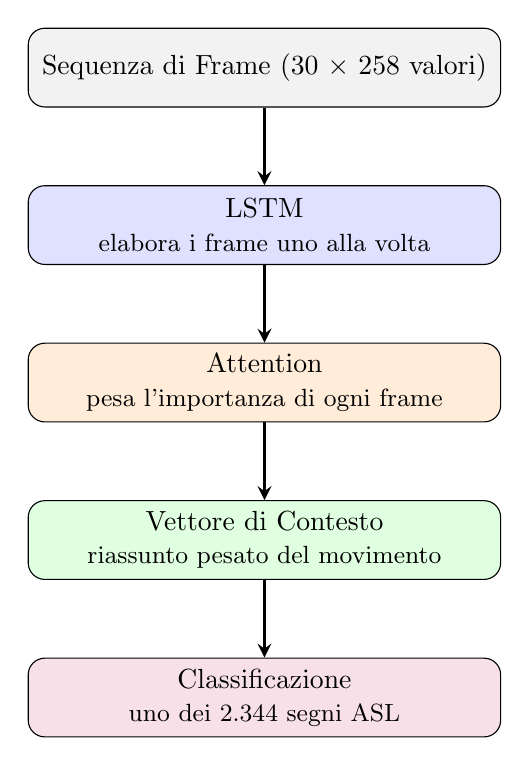
\begin{tikzpicture}[
        box/.style={draw, rounded corners=6pt, minimum width=6cm, minimum height=1cm, font=\normalsize, align=center},
        arr/.style={->, thick, >=stealth, line width=1.2pt}]

        \node[box, fill=gray!10]   (input)  at (0, 0)   {Sequenza di Frame (30 $\times$ 258 valori)};
        \node[box, fill=blue!12]   (lstm)   at (0, -2)  {LSTM \\ {\small elabora i frame uno alla volta}};
        \node[box, fill=orange!15] (att)    at (0, -4)  {Attention \\ {\small pesa l'importanza di ogni frame}};
        \node[box, fill=green!12]  (ctx)    at (0, -6)  {Vettore di Contesto \\ {\small riassunto pesato del movimento}};
        \node[box, fill=purple!12] (cls)    at (0, -8)  {Classificazione \\ {\small uno dei 2.344 segni ASL}};

        \draw[arr] (input) -- (lstm);
        \draw[arr] (lstm)  -- (att);
        \draw[arr] (att)   -- (ctx);
        \draw[arr] (ctx)   -- (cls);

    \end{tikzpicture}
    \caption{Fasi dell'architettura LSTM con Attention: la sequenza viene elaborata dall'LSTM, l'attention seleziona i frame più rilevanti, e il vettore risultante viene usato per la classificazione.}
    \label{fig:lstm_attention}
\end{figure}

\subsection{Confronto e Scelta Finale}

La Tabella~\ref{tab:confronto_architetture} sintetizza il confronto tra le architetture valutate, sulla base di cinque criteri rilevanti per il presente progetto.

\begin{table}[H]
\centering
\begin{tabular}{lccc}
\hline
\textbf{Criterio} & \textbf{LSTM} & \textbf{Transformer} & \textbf{LSTM+Att.} \\
\hline
Modellazione temporale         & Buona    & Ottima     & Buona     \\
Dipendenze a lungo raggio      & Limitata & Eccellente & Buona     \\
Rischio overfitting (32K dati) & Basso    & \textbf{Alto} & Basso     \\
Interpretabilità               & Scarsa   & Limitata   & \textbf{Alta} \\
Complessità implementativa     & Bassa    & Alta       & Media     \\
\hline
\end{tabular}
\caption{Confronto tra architetture neurali per la classificazione di sequenze di landmark.}
\label{tab:confronto_architetture}
\end{table}

La scelta è ricaduta sull'architettura \textbf{LSTM con meccanismo di Attention} per le seguenti ragioni:

\begin{enumerate}
    \item \textbf{Volume di dati limitato:} con 32.435 campioni su 2.344 classi (circa 13.8 campioni per classe), è fondamentale utilizzare un modello con un numero contenuto di parametri. Il Transformer, con la sua architettura multi-layer, rischierebbe di memorizzare i dati di training anziché generalizzare.

    \item \textbf{Sequenze brevi:} le sequenze normalizzate a 30 frame sono sufficientemente corte da non richiedere la capacità di modellazione a lungo raggio del Transformer. L'LSTM è perfettamente in grado di mantenere il contesto su 30 passi temporali.

    \item \textbf{Interpretabilità:} la possibilità di visualizzare i pesi di attention consente di verificare che il modello stia effettivamente ``guardando'' i momenti giusti della sequenza, aggiungendo trasparenza alle decisioni del classificatore.

    \item \textbf{Compatibilità hardware:} l'architettura selezionata è compatibile con le risorse hardware disponibili (GPU NVIDIA RTX 2070, 8 GB VRAM), garantendo tempi di addestramento ragionevoli.
\end{enumerate}
